\documentclass[10pt,landscape]{article}
\usepackage{multicol}
\usepackage[landscape]{geometry}
\usepackage[procnames]{listings}
\usepackage[parfill]{parskip}
\usepackage{fixltx2e}
\usepackage[T1]{fontenc}
\usepackage{lmodern}
\usepackage{graphicx}

% "define" Scala
\usepackage[T1]{fontenc}  
\usepackage[scaled=0.82]{beramono}  
\usepackage{microtype} 

\sbox0{\small\ttfamily A}
\edef\mybasewidth{\the\wd0 }

\lstdefinelanguage{scala}{
  morekeywords={abstract,case,catch,class,def,%
    do,else,extends,false,final,finally,%
    for,if,implicit,import,match,mixin,%
    new,null,object,override,package,%
    private,protected,requires,return,sealed,%
    super,this,throw,trait,true,try,%
    type,val,var,while,with,yield},
  sensitive=true,
  morecomment=[l]{//},
  morecomment=[n]{/*}{*/},
  morestring=[b]",
  morestring=[b]',
  morestring=[b]"""
}

\usepackage{color}
\definecolor{dkgreen}{rgb}{0,0.6,0}
\definecolor{gray}{rgb}{0.5,0.5,0.5}
\definecolor{mauve}{rgb}{0.58,0,0.82}

% Default settings for code listings
\lstset{language=scala,
  showstringspaces=false,
  columns=fixed, % basewidth=\mybasewidth,
  basicstyle={\small\ttfamily},
  numbers=none,
  numberstyle=\footnotesize\color{gray},
  % identifierstyle=\color{red},
  keywordstyle=\color{blue},
  commentstyle=\color{dkgreen},
  stringstyle=\color{mauve},
  breakatwhitespace=true,
  procnamekeys={def, val, var, class, trait, object, extends},
  procnamestyle=\ttfamily\color{red},
}

\lstnewenvironment{scala}
{\lstset{language=scala}}
{}
\lstnewenvironment{cpp}
{\lstset{language=C++}}
{}
\lstnewenvironment{bash}
{\lstset{language=bash}}
{}
\lstnewenvironment{verilog}
{\lstset{language=verilog}}
{}

\newcommand{\isc}{
\lstinline
}

\lstdefinestyle{scala}{language=scala,
  showstringspaces=false,
  columns=fixed, % basewidth=\mybasewidth,
  basicstyle={\small\ttfamily},
  numbers=none,
  numberstyle=\footnotesize\color{gray},
  % identifierstyle=\color{red},
  keywordstyle=\color{blue},
  commentstyle=\color{dkgreen},
  stringstyle=\color{mauve},
  breakatwhitespace=true,
  procnamekeys={def, val, var, class, trait, object, extends},
  procnamestyle=\ttfamily\color{red},
}


% Remove section numbering
\setcounter{secnumdepth}{0}

\geometry{top=.75cm,left=.75cm,right=.75cm,bottom=.75cm}


\pagestyle{empty}
\setlength{\parskip}{0cm}

\makeatletter
\renewcommand{\section}{\@startsection{section}{1}{0mm}%
                                {-2ex plus 4ex}%
                                {-0.01ex plus .01ex}%x
                                {\normalfont\large\bfseries}}
\renewcommand{\subsection}{\@startsection{subsection}{2}{0mm}%
                                {-1ex plus 4ex}%
                                {-0.01ex plus .01ex}%
                                {\normalfont\normalsize\bfseries}}
\renewcommand{\subsubsection}{\@startsection{subsubsection}{3}{0mm}%
                                {-0.01ex plus 0.01ex}%
                                {-0.01ex plus .01ex}%
                                {\normalfont\small\bfseries}}
\makeatother

\begin{document}
\begin{multicols}{3}

\newcommand*\ruleline[1]{\par\noindent\raisebox{.8ex}{\makebox[\linewidth]{\hrulefill\hspace{1ex}\raisebox{-.8ex}{#1}\hspace{1ex}\hrulefill}}}
\renewcommand{\tabcolsep}{.5mm}

\ruleline{\Large{\textbf{Chisel Cheat Sheet}}}
\begin{center}
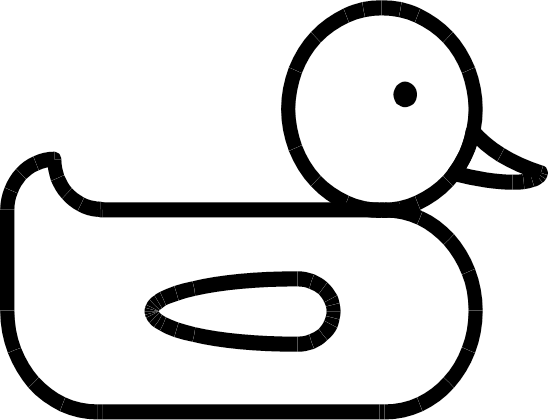
\includegraphics[scale=0.02]{bigduck} Version 0.3 (beta): \today
\end{center}

\fbox{ \parbox{0.95\columnwidth} {
\subsection{Notation In This Document}:
\subsubsection{For Functions and Constructors}: \newline
Arguments given as \texttt{kwd:type} (name and type(s)) \newline
Arguments in brackets (\texttt{[...]}) are optional.
\subsubsection{For Operators}: \newline
\texttt{c}, \texttt{x}, \texttt{y} are of type Chisel \texttt{Data} \newline
\texttt{n}, \texttt{m} are of type Scala \texttt{Int} \newline
\texttt{w(x)}, \texttt{w(y)} are the widths of \texttt{x}, \texttt{y} (respectively) \newline
\texttt{minVal(x)}, \texttt{maxVal(x)} are the minimum or \newline
\phantom{x} maximum possible values of \texttt{x}
} }

\section{Basic Chisel Constructs } \hrulefill
\subsection{Chisel Wire Operators}: \newline
\begin{tabular}{l l}
\verb$val x = UInt()$ & Allocate \verb$a$ as wire of type \verb$UInt()$ \\
\verb$x := y$ & Assign \verb$y$ to wire \verb$x$ \\
\verb$x <> y$ & Connect \verb$x$ and \verb$y$, wire directionality \\
 & is automatically inferred \\
\end{tabular}

\subsection{When } executes blocks conditionally by \verb$Bool$, \newline
\phantom{x} and is equivalent to Verilog \verb$if$
\begin{scala}
when(condition1) {
  // run if condition1 true
} .elsewhen(condition2) {
  // run if condition2 true
} .unless(condition3) {
  // run if condition3 false
} .otherwise {
  // run if none of the above true
}
\end{scala}

\subsection{Switch } executes blocks conditionally by data
\begin{scala}
switch(x) {
  is(value1) {
    // run if x === value1
  } is(value2) {
    // run if x === value2
  }
}
\end{scala}

\subsection{Enum } generates value literals for enumerations \newline
\verb$val s1::s2::$ ... \verb$::sn::Nil$ \newline
\verb$    = Enum(nodeType:UInt, n:Int)$ \newline
\begin{tabular}{l l l}
& \verb$s1$, \verb$s2$, ..., \verb$sn$ & will be created as \verb$nodeType$ literals \\
& & with distinct values \\
& \verb$nodeType$ & type of \verb$s1$, \verb$s2$, ..., \verb$sn$ \\
& \verb$n$ & element count \\
\end{tabular}

\columnbreak

\section{Basic Data Types } \hrulefill
\subsubsection{Constructors}: \newline
\verb$Bool([x:Boolean])$ \newline
\verb$Bits/UInt/SInt([x:Int/String], [width:Int])$ \newline
\begin{tabular}{l l l}
& \verb$x$ & {\em (optional)} create a literal from Scala type/ \\
& & pased \verb$String$, or declare unassigned if missing \\
& \verb$width$ & {\em (optional)} bit width (inferred if missing) \\
\end{tabular}

\subsubsection{Bits, UInt, SInt Casts}: reinterpret cast except for:\newline
\begin{tabular*}{\columnwidth}{@{\extracolsep{\fill} } l l l}
\verb$UInt$ $\rightarrow$ \verb$SInt$ & Zero-extend to SInt & \\
\end{tabular*}

\subsubsection{Bool Operators}: \newline
\begin{tabular*}{\columnwidth}{@{\extracolsep{\fill} } l l l}
Chisel & Explanation & Width \\
\hline
\hline
\verb$!x$ & Logical NOT & \verb$1$ \\
\verb$x && y$ & Logical AND & \verb$1$ \\
\verb$x || y$ & Logical OR & \verb$1$ \\
\end{tabular*}

\subsubsection{Bits Operators}: \newline
\begin{tabular*}{\columnwidth}{@{\extracolsep{\fill} } l l l}
Chisel & Explanation & Width \\
\hline
\hline
\verb$x(n)$ & Extract bit, \verb$0$ is LSB & \verb$1$ \\
\verb$x(n, m)$ & Extract bitfield & \verb$n - m + 1$ \\
\verb$x << y$ & Dynamic left shift & \verb$w(x) + maxVal(y)$ \\
\verb$x >> y$ & Dynamic right shift & \verb$w(x) - minVal(y)$ \\
\verb$x << n$ & Static left shift & \verb$w(x) + n$ \\
\verb$x >> n$ & Static right shift & \verb$w(x) - n$ \\
\verb$Fill(n, x)$ & Replicate \verb$x$, \verb$n$ times & \verb$n * w(x)$ \\
\verb$Cat(x, y)$ & Concatenate bits & \verb$w(x) + w(y)$ \\
\verb$Mux(c, x, y)$ & If \verb$c$: then \verb$x$, else \verb$y$ & \verb$max(w(x), w(y))$ \\
\hline
\verb$~x$ & Bitwise NOT & \verb$w(x)$ \\
\verb$x & y$ & Bitwise AND & \verb$max(w(x), w(y))$ \\
\verb$x | y$ & Bitwise OR & \verb$max(w(x), w(y))$ \\
\verb$x ^ y$ & Bitwise XOR & \verb$max(w(x), w(y))$ \\
\hline
\verb$x === y$ & Equality & \verb$1$ \\
\verb$x != y$ & Inequality & \verb$1$ \\
\hline
\verb$andR(x)$ & AND-reduce & \verb$1$ \\
\verb$orR(x)$ & OR-reduce & \verb$1$ \\
\verb$xorR(x)$ & XOR-reduce & \verb$1$ \\
\end{tabular*}

\subsubsection{UInt, SInt Operators}: (bitwdths given for \verb$UInt$s) \newline
\begin{tabular*}{\columnwidth}{@{\extracolsep{\fill} } l l l}
Chisel & Explanation & Width \\
\hline
\hline
\verb$x + y$ & Addition & \verb$max(w(x), w(y))$ \\
\verb$x - y$ & Subtraction & \verb$max(w(x), w(y))$ \\
\verb$x * y$ & Multiplication & \verb$w(x) + w(y)$ \\
\verb$x / y$ & Division & \verb$w(x)$ \\
\verb$x % y$ & Modulus & \verb$bits(maxVal(y) - 1)$ \\
\hline
\verb$x > y$ & Greater than & \verb$1$ \\
\verb$x >= y$ & Greater than or equal & \verb$1$ \\
\verb$x < y$ & Less than & \verb$1$ \\
\verb$x <= y$ & Less than or equal & \verb$1$ \\
\hline
\verb$x >> y$ & Arithmetic right shift & \verb$w(x) - minVal(y)$ \\
\verb$x >> n$ & Arithmetic right shift & \verb$w(x) - n$ \\
\end{tabular*}

\columnbreak

\section{Aggregate Types } \hrulefill
\subsection{Bundle } contains \verb$Data$ types indexed by name
\subsubsection{Defining}: subclass \verb$Bundle$, define components:
\begin{scala}
class MyBundle extends Bundle {
  val a = Bool()
  val b = UInt(width = 32)
}
\end{scala}
\subsubsection{Constructor}: instantiate \verb$Bundle$ subclass: \newline
\verb$val my_bundle = new MyBundle()$
\subsubsection{Inline defining}: define a \verb$Bundle$ type:
\begin{scala}
val my_bundle = new Bundle {
  val a = Bool()
  val b = UInt(width = 32)
}
\end{scala}
\subsubsection{Using}: access elements through dot notation: \newline
\verb$val bundleVal = my_bundle.a$ \newline
\verb$my_bundle.a := Bool(true)$

\subsection{Vec } is an indexable vector of \verb$Data$ types
\subsubsection{Constructor}: \newline
\verb$val myVec = Vec.fill(n:Int) {gen:Data}$ \newline
\begin{tabular}{l l l}
& \verb$n$ & vector depth (elements) \\
& \verb$gen$ & element data type \\
\end{tabular}
\subsubsection{Using}: access elements by indexing: \newline
\verb$readVal := myVec(ind:Data)$ (dynamic index) \newline
\verb$readVal := myVec(idx:Int)$ (static index) \newline
\verb$myVec(ind:Data) := writeVal$ (dynamic index) \newline
\verb$myVec(idx:Int) := writeVal$ (static index)



\section{Modules } \hrulefill
\subsubsection{Defining}: subclass \verb$Module$ with elements and code: \newline
(\verb$Module$s may be parameterized and hierarchical)
\begin{scala}
class SyncAccum(width:Int) extends Module {
  val io = new Bundle {
    val in = UInt(INPUT,  width)
    val out  = UInt(OUTPUT, width)
  }
  val sum = new Reg(UInt())
  sum := sum + io.in
  io.out := sum
}
\end{scala}
\subsubsection{Usage}: access elements using dot notation: \newline
\phantom{x} (code inside a \verb$Module$ is always running)
\begin{scala}
val my_module = Module(new SyncAccum(32))
my_module.io.in := some_data
val sum := my_module.io.out
\end{scala}

\columnbreak

\section{State Elements } \hrulefill
\subsection{Registers } retain state until updated
\subsubsection{Constructor}: \newline
\verb$val my_reg = Reg([outType:Data], [next:Data],$ \newline
\verb$                 [init:Data])$ \newline
\begin{tabular}{l l l}
& \verb$outType$ & {\em (optional)} register type (or inferred) \\
& \verb$next$ & {\em (optional)} update value every clock \\
& \verb$init$ & {\em (optional)} initialization value on reset \\
\end{tabular}
\subsubsection{Updating}: assign to latch new value on next clock: \newline
\verb$my_reg := next_val$ \newline
The last update (lexically, per clock) runs

\subsection{Read-Write Memory}
\subsubsection{Constructor}: \newline
\verb$val my_mem = Mem(out:Data, n:Int,$ \newline
\verb$                 seqRead:Boolean)$ \newline
\begin{tabular}{l l l}
& \verb$out$ & memory element type \\
& \verb$n$ & memory depth (elements) \\
& \verb$seqRead$ & only update reads on clock edge \\
\end{tabular}
\subsubsection{Using}: access elements by indexing: \newline
\verb$val readVal = mem(addr:UInt/Int)$ \newline
Synchronous read: assign output to \verb$Reg$ \newline
\verb$mem(addr:UInt/Int) := y$

\section{Hardware Generation } \hrulefill
\subsection{Functions } provide block abstractions for code
\subsubsection{Defining}: write Scala functions with Chisel code:
\begin{scala}
def FunAdder(op_a:UInt, op_b:UInt): UInt {
  a + b
}
\end{scala}
\subsubsection{Usage}: hardware is instantiated when called:
\begin{scala}
sum := FunAdder(UInt(1), some_data)
\end{scala}

\subsection{If/For } can be used to control hardware generation \newline
\phantom{x} and is equivalent to Verilog \verb$generate if$/\verb$for$

\section{Standard Library } \hrulefill
\subsection{Decoupled } is a \verb$Bundle$ with a ready-valid interface,\newline
\phantom{x} where the consumer should flip the interface:
\subsubsection{Constructor}: \newline
\verb$val my_readyvalid = Decoupled(type:Data)$ \newline
\begin{tabular}{l l l}
& \verb$type$ & data type \\
\end{tabular}
\subsubsection{Interface}: \newline
\begin{tabular}{l l l}
& \verb$.ready$ & ready \verb$Bool$ \\
& \verb$.valid$ & valid \verb$Bool$ \\
& \verb$.bits$ & data \\
\end{tabular}

\subsection{PipeIO } is a \verb$Bundle$ with a valid interface,\newline
\phantom{x} where the consumer should flip the interface
\subsubsection{Constructor}: \newline
\verb$val my_pipe = PipeIO(type:Data)$ \newline
\begin{tabular}{l l l}
& \verb$type$ & data type \\
\end{tabular}
\subsubsection{Interface}: \newline
\begin{tabular}{l l l}
& \verb$.valid$ & valid \verb$Bool$ \\
& \verb$.bits$ & data \\
\end{tabular}

\subsection{Arbiters } are \verb$Module$s connecting multiple producers\newline
\phantom{x} to one consumer \newline
\verb$Arbiter$ prioritizes lower producers \newline
\verb$RRArbiter$ runs in round-robin order
\subsubsection{Constructor}: \newline
\verb$val arb = Arbiter(gen:Data, n:Int)$ \newline
\begin{tabular}{l l l}
& \verb$gen$ & data type \\
& \verb$n$ & number of producers \\
\end{tabular}
\subsubsection{Interface}: \newline
\begin{tabular}{l l l}
& \verb$.io.in$ & \verb$Vec$ of \verb$Decoupled$ inputs \\
& \verb$.io.out$ & output as \verb$Decoupled$ \\
\end{tabular}

\end{multicols}
\end{document}
